\documentclass{beamer}
\usepackage{beamerthemesplit}
\usepackage{wrapfig}
\usetheme{SPbGU}
\usepackage{pdfpages}
\usepackage{amsmath}
\usepackage{cmap} 
\usepackage[T2A]{fontenc} 
\usepackage[utf8]{inputenc}
\usepackage[english,russian]{babel}
\usepackage{indentfirst}
\usepackage{amsmath}
\usepackage{tikz}
\usepackage{multirow}
\usepackage[noend]{algpseudocode}
\usepackage{algorithm}
\usepackage{algorithmicx}
\usetikzlibrary{shapes,arrows}
%usepackage{fancyvrb}
%\usepackage{minted}
%\usepackage{verbments}


\title[]{YaccConstructor}
\subtitle[YaccConstructor]{Задачи на весенний семестр 2018}
% То, что в квадратных скобках, отображается в левом нижнем углу. 
\institute[]{
Лаборатория языковых инструментов JetBrains \\
Санкт-Петербургский государственный университет \\
Математико-механический факультет }

% То, что в квадратных скобках, отображается в левом нижнем углу.
\author[Семён Григорьев]{Семён Григорьев}

\date{12 февраля 2018г.}

\definecolor{orange}{RGB}{179,36,31}

\begin{document}
{
\begin{frame}[fragile]
  \begin{tabular}{p{2.5cm} p{5.5cm} p{2cm}}
   \begin{center}
      
\includegraphics[height=1.5cm]{pictures/JBLogo3.pdf}
    \end{center}
    &
    \begin{center}
      
\includegraphics[height=1.5cm]{pictures/SPbGU_Logo.png}
    \end{center}
    &
    \begin{center}
      
\includegraphics[height=1.5cm]{pictures/YC_logo.pdf}
    \end{center} 
  \end{tabular}
  \titlepage
\end{frame}
}

\begin{frame}[fragile]
  \transwipe[direction=90]
  \frametitle{YaccConstructor}
  \begin{itemize}
    \item Исследования в области формальных языков
    \item Открытый исходный код
    \begin{itemize}
      \item \url{https://github.com/YaccConstructor}
    \end{itemize}
    \item Основной язык разработки --- F\#
  \end{itemize}
\end{frame}

%\begin{frame}[plain,c]
% \transwipe[direction=90]
% \begin{center}
%  \Huge Применение методов ``машинного обучения'' к классификации цепочек (16s) на основе их вторичной структуры
% \end{center}
%\end{frame}

\begin{frame}[fragile]
\transwipe[direction=90]
\frametitle{Классификация 16s на основе вторичной структуры}
  \begin{itemize}
    \item Задача
    \begin{itemize}
       \item Распознование и классификация микроорганизмов 
    \end{itemize}
    \item Возможное решение
    \begin{itemize}
       \item Использование особенностей вторичной структуры маркерных генов, которая более консервативна, чем первичная
    \end{itemize}
  \end{itemize}
  
\end{frame}

\begin{frame}[fragile]
\transwipe[direction=90]
\frametitle{Вторичная структура}
  
   \begin{center}
      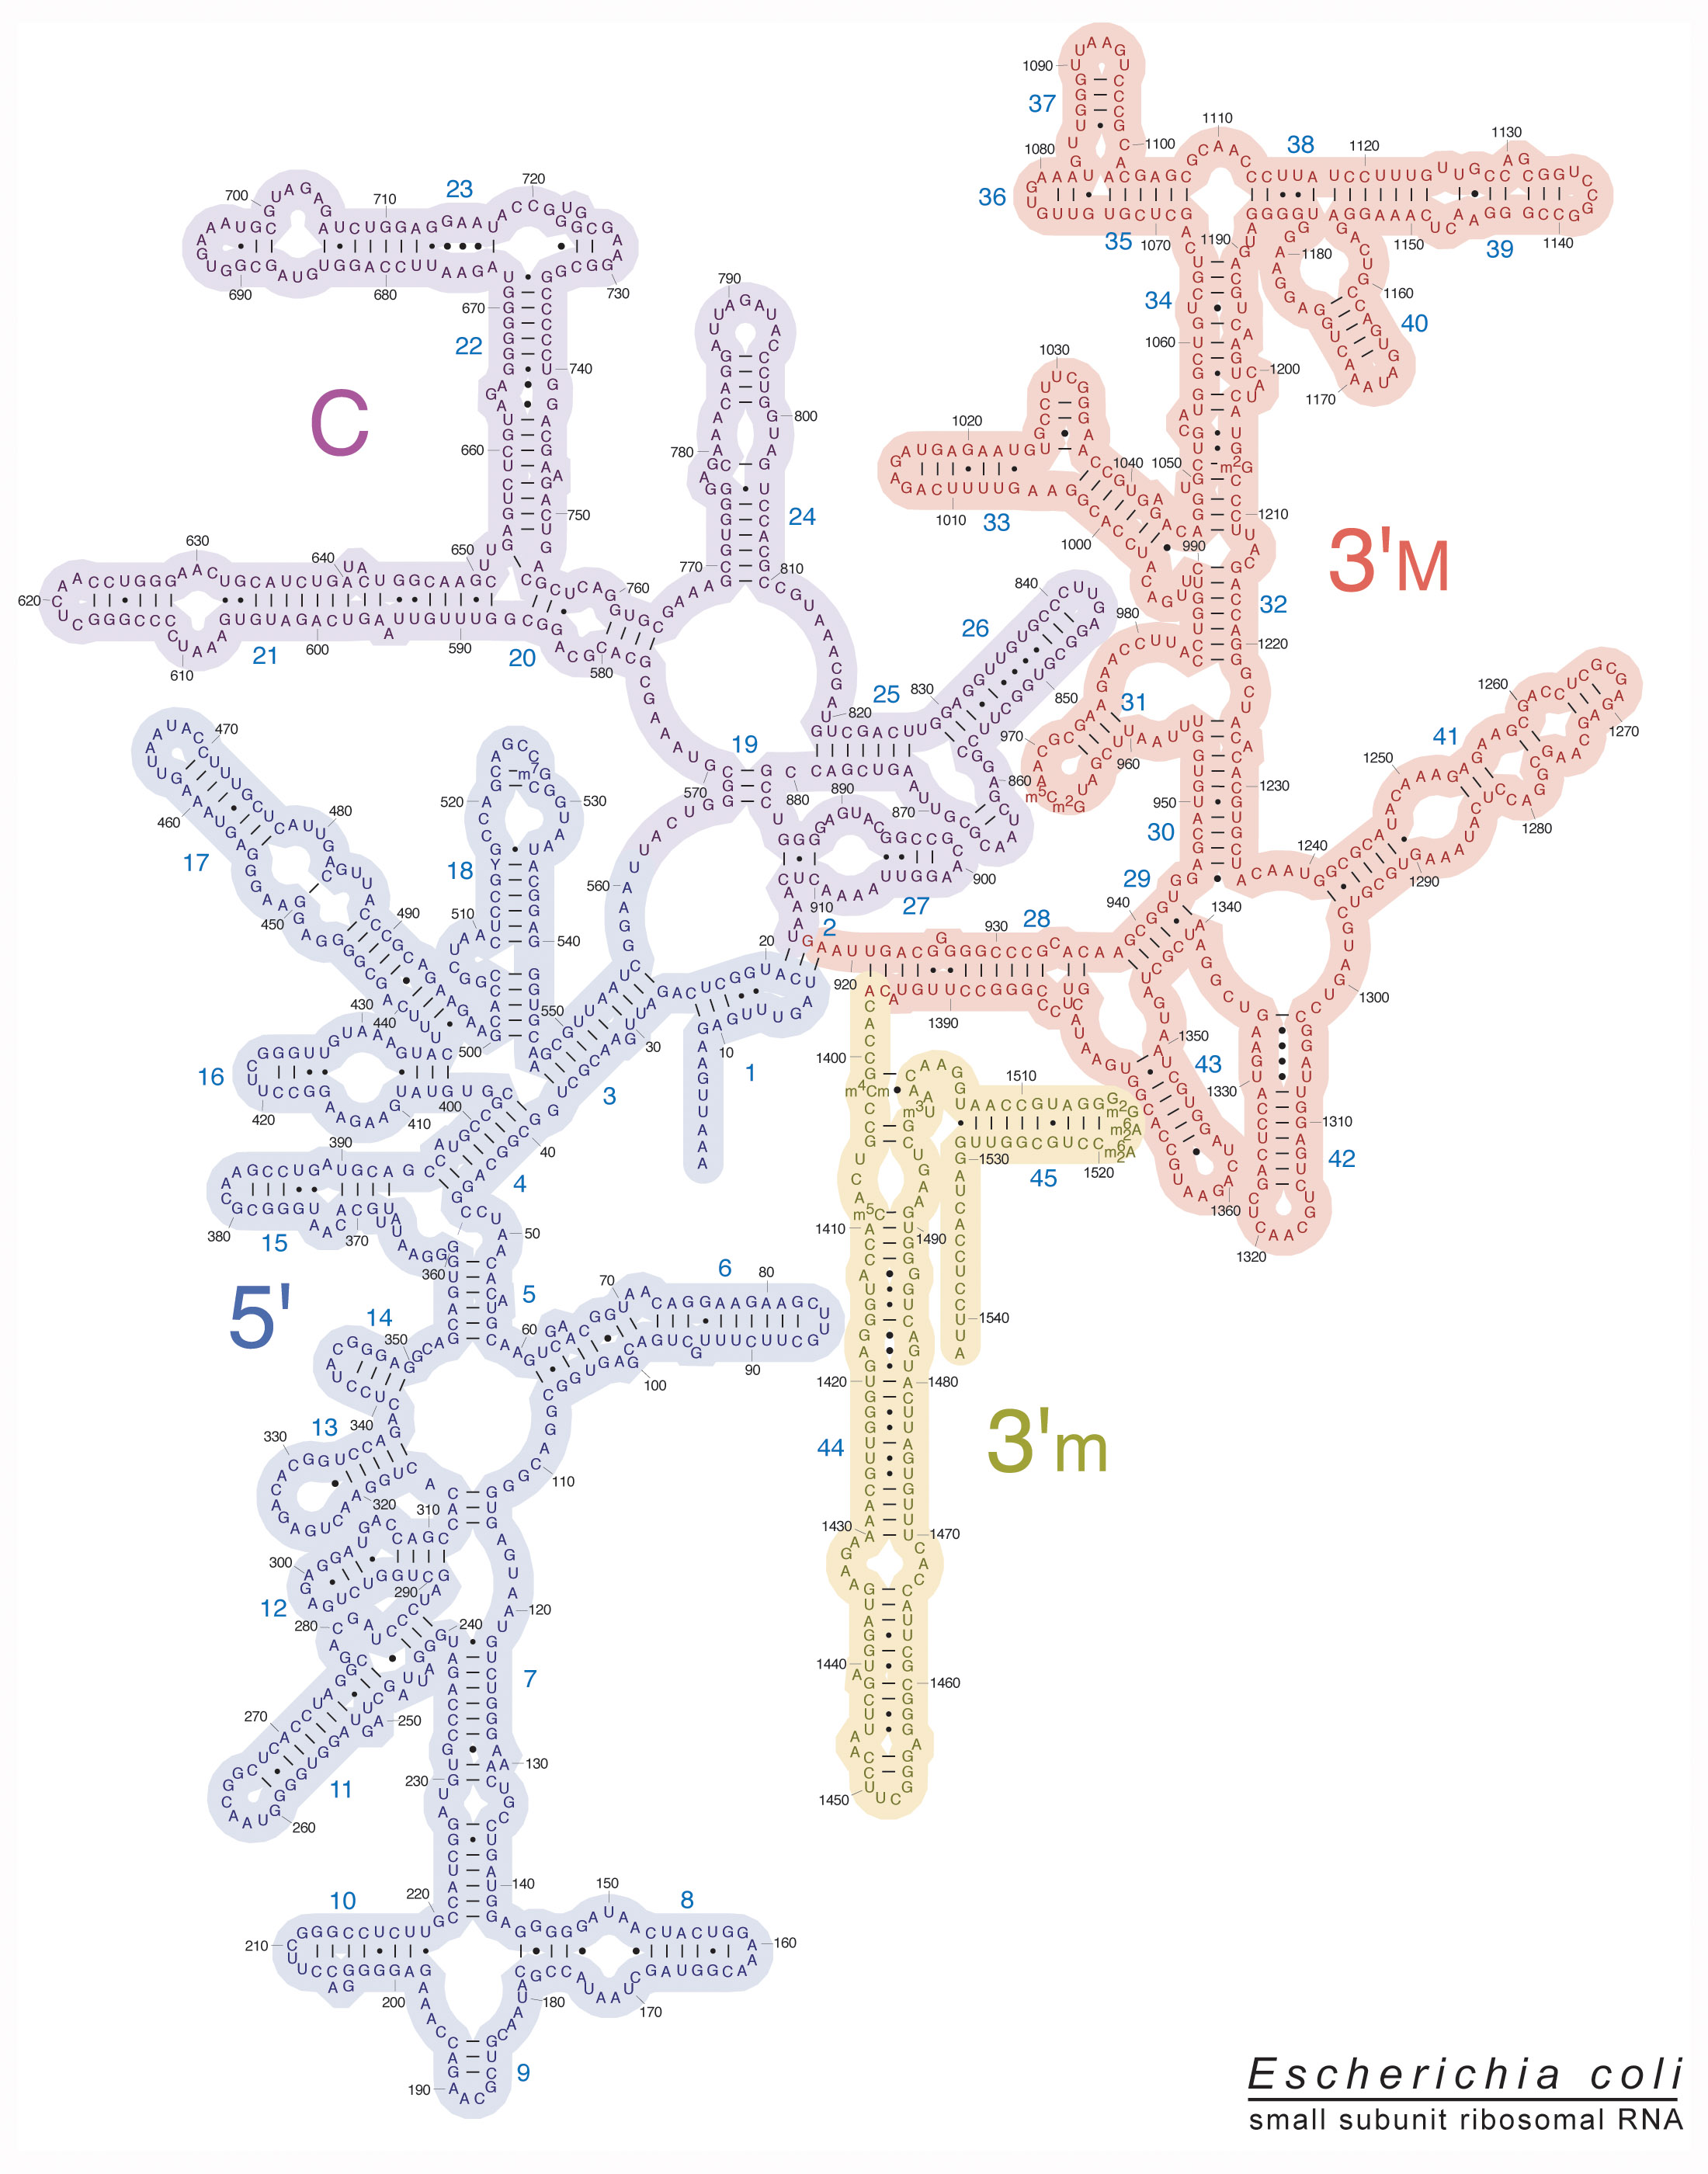
\includegraphics[height=8cm]{pictures/ecoli_16s.jpg}
    \end{center}
  
\end{frame}


\begin{frame}[fragile]
\transwipe[direction=90]
\frametitle{Вторичная структура}
  
  \begin{itemize}
    \item С некоторой точностью может быть описана контекстно-свободной грамматикой
    \item Извлчение особенностей втричной структуры --- синтаксический анализ
    \item Результат может быть представлен в виде битовой матрицы $M$: для фиксированного нетерминала $S$ $M.[i,j] = 1$ если $S \rightarrow^* \omega.[i,j]$
  \end{itemize}
  
\end{frame}



\begin{frame}[fragile]
\transwipe[direction=90]
\frametitle{Примеры матриц}
  \begin{tabular}{p{6cm} p{6cm}}
   \begin{center}
      
\includegraphics[height=5.4cm]{pictures/4.png}
    \end{center}
    &
    \begin{center}
      
\includegraphics[height=5.4cm]{pictures/1.png}
    \end{center}
%    \\
%    \begin{center}
%      
\includegraphics[height=4.4cm]{pictures/3.png}
%    \end{center}
%    &
%    \begin{center}
%      
\includegraphics[height=4.4cm]{pictures/4.png}
%    \end{center}

  \end{tabular}
\end{frame}
      
\begin{frame}[fragile]
\transwipe[direction=90]
\frametitle{Задачи}
\begin{itemize}
\item Обработка химер
\item Интеграция с базой данных Greengenes
\item Извлечение ключевых, с точки зрения нейронной сети, особенностей вторичной структуры
\item Описание задач: \url{https://goo.gl/3jBUKF}
\item Тестовая задача: \url{https://goo.gl/DmGNYs}
\item ``Направления развития'': курсовая, диплом, публикации
\end{itemize}
\end{frame}

\begin{frame}
  \transwipe[direction=90]
  \frametitle{Требования к знаниям и навыкам}
  \begin{itemize}
    \item Методы и алгоритмы обработки данных, статистические методы, машинное обучение, нейронные сети (теория и практика)
    \item Умение читать и понимать научные статьи
    \item Умение читать и понимать чужой код    
  \end{itemize}
\end{frame}
            
\begin{frame}
\transwipe[direction=90]
\frametitle{Контакты}
\begin{itemize}
  \item Почта: \url{rsdpisuy@gmail.com}
  \item Исходный код YaccConstructor: \url{https://github.com/YaccConstructor}
\end{itemize}
\end{frame}
\end{document}
